\documentclass[a4paper,12pt]{article}
\usepackage[margin=2cm]{geometry}
\usepackage[thinfonts]{uglix2}
\usepackage{ulem}
\nouveaustyle
\begin{document}
\titre{Contrôle 01}{NSI2}{10/2021}

{\color{UGLiBlue}\Huge\titlefont Partie 1 : sur papier\\}

\exo{ - Fonction d'Ackermann-Péter\hfill 4pts}\\

Cette fonction est définie pour tout $m\in\N$ et tout $n\in\N$ par
 $$A(m,n)=\begin{cases}
	n+1 & \mbox{si } m=0\\
	A(m-1,1) &\mbox{si } m>0\mbox{ et } n=0\\
	A(m-1,A(m,n-1)) &\mbox{si } m>0\mbox{ et } n>0\\
\end{cases}$$

\'Ecrire la fonction $A$ en \textsc{Python}.\\

\carreauxseyes{16.8}{8.8}\\

\exo{ - Fonction mystère\hfill 4pts}

On considère la fonction suivante:
\pythonfile{scripts/mystery.py}

On rappelle que pour une variable \pythoninline{lst} de type \pythoninline{list}, \pythoninline{lst[:-1]} désigne le \textit{dernier} élément de \pythoninline{lst} et que pour tous \pythoninline{int a} et \pythoninline{b}, \pythoninline{lst[a:b]} désigne la sous-liste extraite de \pythoninline{lst} de
l'élément d'indice \pythoninline{a} \textit{inclus} à celui d'indice \pythoninline{b} \textit{exclu}.

\begin{enumerate}[\bfseries 1.]
	\item 	Que renvoie \pythoninline{mystery([1])} ?\\

    \carreauxseyes{16}{3.2}
	\item 	Que renvoie \pythoninline{mystery([1, 2, 3])} ?\\

    \carreauxseyes{16}{3.2}
    \item   Quel est le rôle de cette fonction ?\\

    \carreauxseyes{16}{3.2}\\
\end{enumerate}


\exo{ - BDD artistique\hfill 3pts}\\

On veut construire une base de données d'\oe uvres artistiques. Voici un résumé des données que l'on a récoltées.\\
Seul le premier tableau n'est pas donné en entier car il comporte trop de lignes.\\
Donner le modèle relationnel en ligne de la BDD. Ne pas oublier d'indiquer les types des attributs, de souligner en trait plein les clés primaires et en pointillés les clés étrangères.\\
\newpage
\begin{center}
\textbf{Œuvre}\\[1em]

\begin{tabular}{|c|c|c|c|c|}
\hline
\rowcolor{UGLiOrange} \textbf{\color{white}id} &\textbf{\color{white}titre}&\textbf{\color{white}creation}&\textbf{\color{white}id\_categorie}&\textbf{\color{white}id\_artiste}\\
\hline
130&Cheval et cavalier &1511 &5 &40\\
196&Colombe de la paix &1949 &2 &56\\
454&Guernica &1937&4&56\\
546&L'Homme de Vitruve&1490&2&40\\
591&L'escalier de Chambord&1516&3&40\\
634&La Cène&1498&4&40\\
649&Les Éléphants&1948&4&78\\
685&La Girafe en feu&1937&4&78\\
706&La Joconde&1519&4&40\\
...&... & ... & ... & ...\\
\hline
\end{tabular}\\[2em]

\textbf{Artiste}\\[1em]

\begin{tabular}{|c|c|c|c|}
\hline
\rowcolor{UGLiOrange} \textbf{\color{white}id} &\textbf{\color{white}nom}&\textbf{\color{white}naissance}&\textbf{\color{white}mort}\\
\hline
40 & Léonard de Vinci & 1452 & 1519\\
56 & Pablo Picasso & 1881 & 1973 \\
78 & Salvador Dali & 1904 & 1989\\
\hline
\end{tabular}\\[2em]

\textbf{Catégorie}\\[1em]

\begin{tabular}{|c|c|}
\hline
\rowcolor{UGLiOrange} \textbf{\color{white}id} &\textbf{\color{white}classement}\\
\hline
1 & céramique \\
2 & dessin \\
3 & objet \\
4 & peinture \\
5 & sculpture \\
\hline
\end{tabular}
\end{center}\ \\


\carreauxseyes{16}{5.6}
\newpage
\exo{ - CinéHit, c'est plus de hits !\hfill 16pts}


Voici le schéma relationnel de la base de données du site de cinéphiles CinéHit :\\

\begin{encadrecolore}{Schéma relationnel}{UGLiGreen}

\begin{enumerate}[\textbullet]
	\item 	\textbf{Realisateur}(\uline{id\_realisateur INTEGER}, nom VARCHAR(48))\\
	\item 	\scriptsize\textbf{Internaute}(\uline{id\_internaute INTEGER}, prenom VARCHAR(32), nom VARCHAR(32), inscription DATE, email VARCHAR(64))\\\normalsize
            Avec la contrainte utilisateur que l'inscription est postérieure à \texttt{2003-01-01} et que l'email est unique.\\
    \item   \textbf{Genre}(\uline{id\_genre INTEGER}, categorie VARCHAR(24))\\
            Avec la contrainte que la catégorie est unique.\\

     \item  \scriptsize\textbf{Film}(\uline{id\_film INTEGER}, titre VARCHAR(128), sortie DATE, duree INTEGER, \dashuline{genre INTEGER}, \dashuline{realisateur INTEGER}, moyenne DECIMAL)\\\normalsize
     Avec la contrainte que la sortie est postérieure à 1895.\\
     La clé étrangère genre référence la clé primaire id\_genre de la relation \textbf{Genre}, et la clé étrangère realisateur référence la clé primaire id\_realisateur de la relation \textbf{Realisateur}.\\
     L'attribut duree est la durée du film convertie en minutes, et l'attribut moyenne est un nombre décimal entre 0 et 10 et comportant un chiffre après la virgule.\\
     \item \textbf{Note}(\uline{\dashuline{film INTEGER}, \dashuline{internaute INTEGER}}, points INTEGER)\\
     Avec la contrainte que les points sont entre 0 et 10.\\
     La clé primaire est le couple (film, internaute) formé de la clé étrangère film qui référence la clé primaire id\_film de la relation \textbf{Film} et la clé étrangère internaute qui référence la clé id\_internaute  de la relation \textbf{Internaute}.

\end{enumerate}






\end{encadrecolore}
On peut résumer tout ceci par le diagramme ci-dessous.


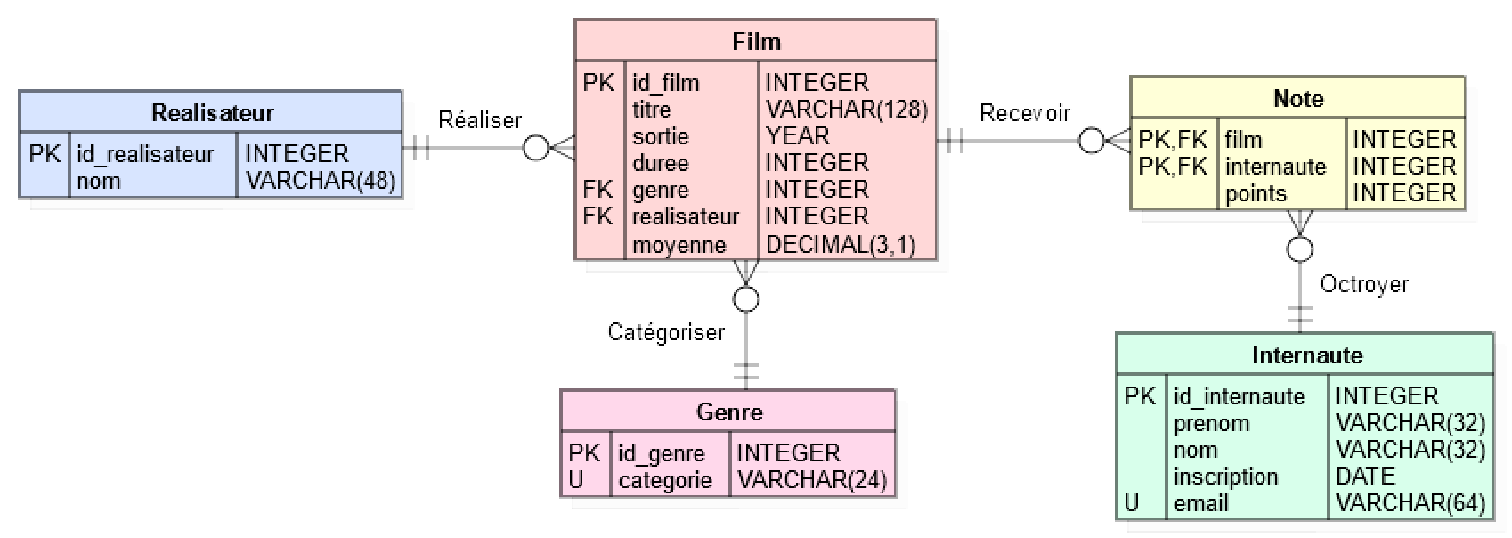
\includegraphics[width=16cm]{img/uml}

\begin{enumerate}[\bfseries 1.]
	\item Que fait la requête \mintinline{sql}{SELECT categorie FROM Genre;} ?\\

    \carreauxseyes{16}{1.6}

	\item Que fait la requête \mintinline{sql}{SELECT * FROM Realisateur WHERE nom LIKE 'Jean%';} ?\\

    \carreauxseyes{16}{1.6}


    \item Que fait la requête suivante ?
            \begin{minted}{sql}
SELECT titre,categorie
FROM Film
    JOIN Genre ON Film(genre) = Genre(id_genre);
            \end{minted}
\carreauxseyes{16}{2.4}

\item Quelle requête donne la table complète des films sortis en 1984 ?\\

\carreauxseyes{16}{3.2}

\item Quelle requête donne la table complète des internautes inscrits entre début 2018 et fin 2019 ?\\

\carreauxseyes{16}{3.2}
\newpage
\item Quelle requête donne la table des titres et moyenne des films durant au moins 3h ?\\

\carreauxseyes{16}{4}

\item Quelle requête donne la table des titres des films sortis après 2000 et dont la moyenne est supérieure à 8 ?\\

\carreauxseyes{16}{4}

\item  Quelle requête donne la table complète des films d'Alfred Hitchcock ?\\

\carreauxseyes{16}{4}
\item  Quelle requête donne la table donnant l'identifiant, le titre et l'année de sortie des thrillers ?\\

\carreauxseyes{16}{4}
\newpage
\item  Quelle requête donne la table des noms de réalisateurs et titres de films dont la moyenne est 8.5 ou plus ?\\

\carreauxseyes{16}{4}

\item  Quelle requête donne la table des prénoms et noms des internautes ayant octroyé 1 seul point à un film,
en supprimant les doublons ?\\

\carreauxseyes{16}{4}

\item Quelle requête donne la table des adresses email et des points des internautes qui ont notés « Les Profs » ?\\

\carreauxseyes{16}{4}

\item La requête suivante échoue. Émettre une hypothèse pour expliquer cet échec.\\
\mintinline{sql}{INSERT INTO Note VALUES(248, 93, 17);}\\

\carreauxseyes{16}{4}

\item Expliquer pourquoi la requête suivante échoue :\\
\mintinline{sql}{DELETE FROM Internaute WHERE id_internaute = 50;}\\

\carreauxseyes{16}{4}

\item Donner les requêtes SQL permettant d'inscrire l'utilisateur et le film suivant :\\
Léo Part s'est inscrit sur le site le 21 juin 2020 avec l'adresse mail \texttt{leo.part@alapla.ge}. Il a l'identifiant 104.\\
Il a mis la note de 9 sur 10 au film de science-fiction « Contact » de Robert Zemeckis qui est sorti en 1997 et qui dure 2 h 33 min.\\
Le genre de ce film est 13 et son identifiant 694.\\

\carreauxseyes{16}{6.4}

\item Donner les requêtes SQL afin de supprimer le film « Fatal » de la BDD du site CinéHit tout en maintenant son intégrité. L'identifiant du film est 446.\\

\carreauxseyes{16}{6.4}
\end{enumerate}
\end{document}
